% This file was created by matplotlib2tikz v0.6.0.
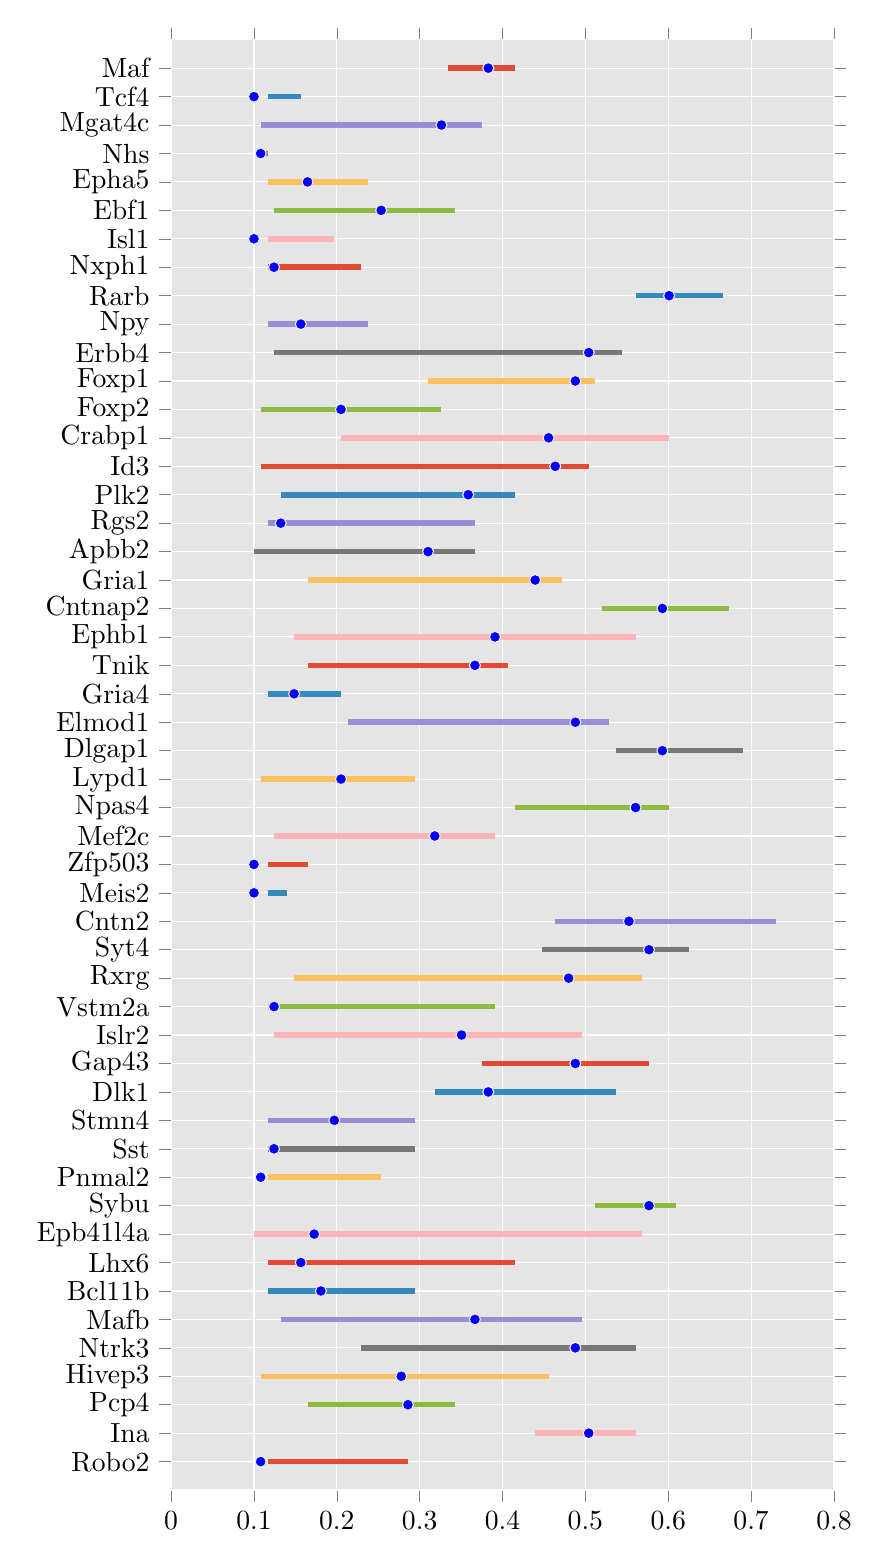
\begin{tikzpicture}

\definecolor{color3}{rgb}{0.984313725490196,0.756862745098039,0.368627450980392}
\definecolor{color5}{rgb}{1,0.709803921568627,0.72156862745098}
\definecolor{color2}{rgb}{0.596078431372549,0.556862745098039,0.835294117647059}
\definecolor{color1}{rgb}{0.203921568627451,0.541176470588235,0.741176470588235}
\definecolor{color0}{rgb}{0.886274509803922,0.290196078431373,0.2}
\definecolor{color4}{rgb}{0.556862745098039,0.729411764705882,0.258823529411765}

\begin{axis}[
xmin=0, xmax=0.8,
ymin=-1, ymax=50,
width=10cm,
height=20cm,
ytick={0,1,2,3,4,5,6,7,8,9,10,11,12,13,14,15,16,17,18,19,20,21,22,23,24,25,26,27,28,29,30,31,32,33,34,35,36,37,38,39,40,41,42,43,44,45,46,47,48,49},
yticklabels={Robo2,Ina,Pcp4,Hivep3,Ntrk3,Mafb,Bcl11b,Lhx6,Epb41l4a,Sybu,Pnmal2,Sst,Stmn4,Dlk1,Gap43,Islr2,Vstm2a,Rxrg,Syt4,Cntn2,Meis2,Zfp503,Mef2c,Npas4,Lypd1,Dlgap1,Elmod1,Gria4,Tnik,Ephb1,Cntnap2,Gria1,Apbb2,Rgs2,Plk2,Id3,Crabp1,Foxp2,Foxp1,Erbb4,Npy,Rarb,Nxph1,Isl1,Ebf1,Epha5,Nhs,Mgat4c,Tcf4,Maf},
tick align=outside,
xmajorgrids,
x grid style={white},
ymajorgrids,
y grid style={white},
axis line style={white},
axis background/.style={fill=white!89.803921568627459!black}
]
\addplot [only marks, draw=white!93.333333333333329!black, fill=blue, colormap={mymap}{[1pt]
  rgb(0pt)=(0,0,0.5);
  rgb(22pt)=(0,0,1);
  rgb(25pt)=(0,0,1);
  rgb(68pt)=(0,0.86,1);
  rgb(70pt)=(0,0.9,0.967741935483871);
  rgb(75pt)=(0.0806451612903226,1,0.887096774193548);
  rgb(128pt)=(0.935483870967742,1,0.0322580645161291);
  rgb(130pt)=(0.967741935483871,0.962962962962963,0);
  rgb(132pt)=(1,0.925925925925926,0);
  rgb(178pt)=(1,0.0740740740740741,0);
  rgb(182pt)=(0.909090909090909,0,0);
  rgb(200pt)=(0.5,0,0)
}, visualization depends on={\thisrow{sizedata} \as\perpointmarksize}, scatter/@pre marker code/.append style={/tikz/mark size=\perpointmarksize}]
table {%
x                      y                      sizedata
+3.828282828282829e-01 +4.900000000000000e+01 +5.641895835477563e+00
};
\addplot [only marks, draw=white!93.333333333333329!black, fill=blue, colormap={mymap}{[1pt]
  rgb(0pt)=(0,0,0.5);
  rgb(22pt)=(0,0,1);
  rgb(25pt)=(0,0,1);
  rgb(68pt)=(0,0.86,1);
  rgb(70pt)=(0,0.9,0.967741935483871);
  rgb(75pt)=(0.0806451612903226,1,0.887096774193548);
  rgb(128pt)=(0.935483870967742,1,0.0322580645161291);
  rgb(130pt)=(0.967741935483871,0.962962962962963,0);
  rgb(132pt)=(1,0.925925925925926,0);
  rgb(178pt)=(1,0.0740740740740741,0);
  rgb(182pt)=(0.909090909090909,0,0);
  rgb(200pt)=(0.5,0,0)
}, visualization depends on={\thisrow{sizedata} \as\perpointmarksize}, scatter/@pre marker code/.append style={/tikz/mark size=\perpointmarksize}]
table {%
x                      y                      sizedata
+1.000000000000000e-01 +4.800000000000000e+01 +5.641895835477563e+00
};
\addplot [only marks, draw=white!93.333333333333329!black, fill=blue, colormap={mymap}{[1pt]
  rgb(0pt)=(0,0,0.5);
  rgb(22pt)=(0,0,1);
  rgb(25pt)=(0,0,1);
  rgb(68pt)=(0,0.86,1);
  rgb(70pt)=(0,0.9,0.967741935483871);
  rgb(75pt)=(0.0806451612903226,1,0.887096774193548);
  rgb(128pt)=(0.935483870967742,1,0.0322580645161291);
  rgb(130pt)=(0.967741935483871,0.962962962962963,0);
  rgb(132pt)=(1,0.925925925925926,0);
  rgb(178pt)=(1,0.0740740740740741,0);
  rgb(182pt)=(0.909090909090909,0,0);
  rgb(200pt)=(0.5,0,0)
}, visualization depends on={\thisrow{sizedata} \as\perpointmarksize}, scatter/@pre marker code/.append style={/tikz/mark size=\perpointmarksize}]
table {%
x                      y                      sizedata
+3.262626262626263e-01 +4.700000000000000e+01 +5.641895835477563e+00
};
\addplot [only marks, draw=white!93.333333333333329!black, fill=blue, colormap={mymap}{[1pt]
  rgb(0pt)=(0,0,0.5);
  rgb(22pt)=(0,0,1);
  rgb(25pt)=(0,0,1);
  rgb(68pt)=(0,0.86,1);
  rgb(70pt)=(0,0.9,0.967741935483871);
  rgb(75pt)=(0.0806451612903226,1,0.887096774193548);
  rgb(128pt)=(0.935483870967742,1,0.0322580645161291);
  rgb(130pt)=(0.967741935483871,0.962962962962963,0);
  rgb(132pt)=(1,0.925925925925926,0);
  rgb(178pt)=(1,0.0740740740740741,0);
  rgb(182pt)=(0.909090909090909,0,0);
  rgb(200pt)=(0.5,0,0)
}, visualization depends on={\thisrow{sizedata} \as\perpointmarksize}, scatter/@pre marker code/.append style={/tikz/mark size=\perpointmarksize}]
table {%
x                      y                      sizedata
+1.080808080808081e-01 +4.600000000000000e+01 +5.641895835477563e+00
};
\addplot [only marks, draw=white!93.333333333333329!black, fill=blue, colormap={mymap}{[1pt]
  rgb(0pt)=(0,0,0.5);
  rgb(22pt)=(0,0,1);
  rgb(25pt)=(0,0,1);
  rgb(68pt)=(0,0.86,1);
  rgb(70pt)=(0,0.9,0.967741935483871);
  rgb(75pt)=(0.0806451612903226,1,0.887096774193548);
  rgb(128pt)=(0.935483870967742,1,0.0322580645161291);
  rgb(130pt)=(0.967741935483871,0.962962962962963,0);
  rgb(132pt)=(1,0.925925925925926,0);
  rgb(178pt)=(1,0.0740740740740741,0);
  rgb(182pt)=(0.909090909090909,0,0);
  rgb(200pt)=(0.5,0,0)
}, visualization depends on={\thisrow{sizedata} \as\perpointmarksize}, scatter/@pre marker code/.append style={/tikz/mark size=\perpointmarksize}]
table {%
x                      y                      sizedata
+1.646464646464647e-01 +4.500000000000000e+01 +5.641895835477563e+00
};
\addplot [only marks, draw=white!93.333333333333329!black, fill=blue, colormap={mymap}{[1pt]
  rgb(0pt)=(0,0,0.5);
  rgb(22pt)=(0,0,1);
  rgb(25pt)=(0,0,1);
  rgb(68pt)=(0,0.86,1);
  rgb(70pt)=(0,0.9,0.967741935483871);
  rgb(75pt)=(0.0806451612903226,1,0.887096774193548);
  rgb(128pt)=(0.935483870967742,1,0.0322580645161291);
  rgb(130pt)=(0.967741935483871,0.962962962962963,0);
  rgb(132pt)=(1,0.925925925925926,0);
  rgb(178pt)=(1,0.0740740740740741,0);
  rgb(182pt)=(0.909090909090909,0,0);
  rgb(200pt)=(0.5,0,0)
}, visualization depends on={\thisrow{sizedata} \as\perpointmarksize}, scatter/@pre marker code/.append style={/tikz/mark size=\perpointmarksize}]
table {%
x                      y                      sizedata
+2.535353535353535e-01 +4.400000000000000e+01 +5.641895835477563e+00
};
\addplot [only marks, draw=white!93.333333333333329!black, fill=blue, colormap={mymap}{[1pt]
  rgb(0pt)=(0,0,0.5);
  rgb(22pt)=(0,0,1);
  rgb(25pt)=(0,0,1);
  rgb(68pt)=(0,0.86,1);
  rgb(70pt)=(0,0.9,0.967741935483871);
  rgb(75pt)=(0.0806451612903226,1,0.887096774193548);
  rgb(128pt)=(0.935483870967742,1,0.0322580645161291);
  rgb(130pt)=(0.967741935483871,0.962962962962963,0);
  rgb(132pt)=(1,0.925925925925926,0);
  rgb(178pt)=(1,0.0740740740740741,0);
  rgb(182pt)=(0.909090909090909,0,0);
  rgb(200pt)=(0.5,0,0)
}, visualization depends on={\thisrow{sizedata} \as\perpointmarksize}, scatter/@pre marker code/.append style={/tikz/mark size=\perpointmarksize}]
table {%
x                      y                      sizedata
+1.000000000000000e-01 +4.300000000000000e+01 +5.641895835477563e+00
};
\addplot [only marks, draw=white!93.333333333333329!black, fill=blue, colormap={mymap}{[1pt]
  rgb(0pt)=(0,0,0.5);
  rgb(22pt)=(0,0,1);
  rgb(25pt)=(0,0,1);
  rgb(68pt)=(0,0.86,1);
  rgb(70pt)=(0,0.9,0.967741935483871);
  rgb(75pt)=(0.0806451612903226,1,0.887096774193548);
  rgb(128pt)=(0.935483870967742,1,0.0322580645161291);
  rgb(130pt)=(0.967741935483871,0.962962962962963,0);
  rgb(132pt)=(1,0.925925925925926,0);
  rgb(178pt)=(1,0.0740740740740741,0);
  rgb(182pt)=(0.909090909090909,0,0);
  rgb(200pt)=(0.5,0,0)
}, visualization depends on={\thisrow{sizedata} \as\perpointmarksize}, scatter/@pre marker code/.append style={/tikz/mark size=\perpointmarksize}]
table {%
x                      y                      sizedata
+1.242424242424243e-01 +4.200000000000000e+01 +5.641895835477563e+00
};
\addplot [only marks, draw=white!93.333333333333329!black, fill=blue, colormap={mymap}{[1pt]
  rgb(0pt)=(0,0,0.5);
  rgb(22pt)=(0,0,1);
  rgb(25pt)=(0,0,1);
  rgb(68pt)=(0,0.86,1);
  rgb(70pt)=(0,0.9,0.967741935483871);
  rgb(75pt)=(0.0806451612903226,1,0.887096774193548);
  rgb(128pt)=(0.935483870967742,1,0.0322580645161291);
  rgb(130pt)=(0.967741935483871,0.962962962962963,0);
  rgb(132pt)=(1,0.925925925925926,0);
  rgb(178pt)=(1,0.0740740740740741,0);
  rgb(182pt)=(0.909090909090909,0,0);
  rgb(200pt)=(0.5,0,0)
}, visualization depends on={\thisrow{sizedata} \as\perpointmarksize}, scatter/@pre marker code/.append style={/tikz/mark size=\perpointmarksize}]
table {%
x                      y                      sizedata
+6.010101010101010e-01 +4.100000000000000e+01 +5.641895835477563e+00
};
\addplot [only marks, draw=white!93.333333333333329!black, fill=blue, colormap={mymap}{[1pt]
  rgb(0pt)=(0,0,0.5);
  rgb(22pt)=(0,0,1);
  rgb(25pt)=(0,0,1);
  rgb(68pt)=(0,0.86,1);
  rgb(70pt)=(0,0.9,0.967741935483871);
  rgb(75pt)=(0.0806451612903226,1,0.887096774193548);
  rgb(128pt)=(0.935483870967742,1,0.0322580645161291);
  rgb(130pt)=(0.967741935483871,0.962962962962963,0);
  rgb(132pt)=(1,0.925925925925926,0);
  rgb(178pt)=(1,0.0740740740740741,0);
  rgb(182pt)=(0.909090909090909,0,0);
  rgb(200pt)=(0.5,0,0)
}, visualization depends on={\thisrow{sizedata} \as\perpointmarksize}, scatter/@pre marker code/.append style={/tikz/mark size=\perpointmarksize}]
table {%
x                      y                      sizedata
+1.565656565656566e-01 +4.000000000000000e+01 +5.641895835477563e+00
};
\addplot [only marks, draw=white!93.333333333333329!black, fill=blue, colormap={mymap}{[1pt]
  rgb(0pt)=(0,0,0.5);
  rgb(22pt)=(0,0,1);
  rgb(25pt)=(0,0,1);
  rgb(68pt)=(0,0.86,1);
  rgb(70pt)=(0,0.9,0.967741935483871);
  rgb(75pt)=(0.0806451612903226,1,0.887096774193548);
  rgb(128pt)=(0.935483870967742,1,0.0322580645161291);
  rgb(130pt)=(0.967741935483871,0.962962962962963,0);
  rgb(132pt)=(1,0.925925925925926,0);
  rgb(178pt)=(1,0.0740740740740741,0);
  rgb(182pt)=(0.909090909090909,0,0);
  rgb(200pt)=(0.5,0,0)
}, visualization depends on={\thisrow{sizedata} \as\perpointmarksize}, scatter/@pre marker code/.append style={/tikz/mark size=\perpointmarksize}]
table {%
x                      y                      sizedata
+5.040404040404041e-01 +3.900000000000000e+01 +5.641895835477563e+00
};
\addplot [only marks, draw=white!93.333333333333329!black, fill=blue, colormap={mymap}{[1pt]
  rgb(0pt)=(0,0,0.5);
  rgb(22pt)=(0,0,1);
  rgb(25pt)=(0,0,1);
  rgb(68pt)=(0,0.86,1);
  rgb(70pt)=(0,0.9,0.967741935483871);
  rgb(75pt)=(0.0806451612903226,1,0.887096774193548);
  rgb(128pt)=(0.935483870967742,1,0.0322580645161291);
  rgb(130pt)=(0.967741935483871,0.962962962962963,0);
  rgb(132pt)=(1,0.925925925925926,0);
  rgb(178pt)=(1,0.0740740740740741,0);
  rgb(182pt)=(0.909090909090909,0,0);
  rgb(200pt)=(0.5,0,0)
}, visualization depends on={\thisrow{sizedata} \as\perpointmarksize}, scatter/@pre marker code/.append style={/tikz/mark size=\perpointmarksize}]
table {%
x                      y                      sizedata
+4.878787878787879e-01 +3.800000000000000e+01 +5.641895835477563e+00
};
\addplot [only marks, draw=white!93.333333333333329!black, fill=blue, colormap={mymap}{[1pt]
  rgb(0pt)=(0,0,0.5);
  rgb(22pt)=(0,0,1);
  rgb(25pt)=(0,0,1);
  rgb(68pt)=(0,0.86,1);
  rgb(70pt)=(0,0.9,0.967741935483871);
  rgb(75pt)=(0.0806451612903226,1,0.887096774193548);
  rgb(128pt)=(0.935483870967742,1,0.0322580645161291);
  rgb(130pt)=(0.967741935483871,0.962962962962963,0);
  rgb(132pt)=(1,0.925925925925926,0);
  rgb(178pt)=(1,0.0740740740740741,0);
  rgb(182pt)=(0.909090909090909,0,0);
  rgb(200pt)=(0.5,0,0)
}, visualization depends on={\thisrow{sizedata} \as\perpointmarksize}, scatter/@pre marker code/.append style={/tikz/mark size=\perpointmarksize}]
table {%
x                      y                      sizedata
+2.050505050505050e-01 +3.700000000000000e+01 +5.641895835477563e+00
};
\addplot [only marks, draw=white!93.333333333333329!black, fill=blue, colormap={mymap}{[1pt]
  rgb(0pt)=(0,0,0.5);
  rgb(22pt)=(0,0,1);
  rgb(25pt)=(0,0,1);
  rgb(68pt)=(0,0.86,1);
  rgb(70pt)=(0,0.9,0.967741935483871);
  rgb(75pt)=(0.0806451612903226,1,0.887096774193548);
  rgb(128pt)=(0.935483870967742,1,0.0322580645161291);
  rgb(130pt)=(0.967741935483871,0.962962962962963,0);
  rgb(132pt)=(1,0.925925925925926,0);
  rgb(178pt)=(1,0.0740740740740741,0);
  rgb(182pt)=(0.909090909090909,0,0);
  rgb(200pt)=(0.5,0,0)
}, visualization depends on={\thisrow{sizedata} \as\perpointmarksize}, scatter/@pre marker code/.append style={/tikz/mark size=\perpointmarksize}]
table {%
x                      y                      sizedata
+4.555555555555556e-01 +3.600000000000000e+01 +5.641895835477563e+00
};
\addplot [only marks, draw=white!93.333333333333329!black, fill=blue, colormap={mymap}{[1pt]
  rgb(0pt)=(0,0,0.5);
  rgb(22pt)=(0,0,1);
  rgb(25pt)=(0,0,1);
  rgb(68pt)=(0,0.86,1);
  rgb(70pt)=(0,0.9,0.967741935483871);
  rgb(75pt)=(0.0806451612903226,1,0.887096774193548);
  rgb(128pt)=(0.935483870967742,1,0.0322580645161291);
  rgb(130pt)=(0.967741935483871,0.962962962962963,0);
  rgb(132pt)=(1,0.925925925925926,0);
  rgb(178pt)=(1,0.0740740740740741,0);
  rgb(182pt)=(0.909090909090909,0,0);
  rgb(200pt)=(0.5,0,0)
}, visualization depends on={\thisrow{sizedata} \as\perpointmarksize}, scatter/@pre marker code/.append style={/tikz/mark size=\perpointmarksize}]
table {%
x                      y                      sizedata
+4.636363636363636e-01 +3.500000000000000e+01 +5.641895835477563e+00
};
\addplot [only marks, draw=white!93.333333333333329!black, fill=blue, colormap={mymap}{[1pt]
  rgb(0pt)=(0,0,0.5);
  rgb(22pt)=(0,0,1);
  rgb(25pt)=(0,0,1);
  rgb(68pt)=(0,0.86,1);
  rgb(70pt)=(0,0.9,0.967741935483871);
  rgb(75pt)=(0.0806451612903226,1,0.887096774193548);
  rgb(128pt)=(0.935483870967742,1,0.0322580645161291);
  rgb(130pt)=(0.967741935483871,0.962962962962963,0);
  rgb(132pt)=(1,0.925925925925926,0);
  rgb(178pt)=(1,0.0740740740740741,0);
  rgb(182pt)=(0.909090909090909,0,0);
  rgb(200pt)=(0.5,0,0)
}, visualization depends on={\thisrow{sizedata} \as\perpointmarksize}, scatter/@pre marker code/.append style={/tikz/mark size=\perpointmarksize}]
table {%
x                      y                      sizedata
+3.585858585858586e-01 +3.400000000000000e+01 +5.641895835477563e+00
};
\addplot [only marks, draw=white!93.333333333333329!black, fill=blue, colormap={mymap}{[1pt]
  rgb(0pt)=(0,0,0.5);
  rgb(22pt)=(0,0,1);
  rgb(25pt)=(0,0,1);
  rgb(68pt)=(0,0.86,1);
  rgb(70pt)=(0,0.9,0.967741935483871);
  rgb(75pt)=(0.0806451612903226,1,0.887096774193548);
  rgb(128pt)=(0.935483870967742,1,0.0322580645161291);
  rgb(130pt)=(0.967741935483871,0.962962962962963,0);
  rgb(132pt)=(1,0.925925925925926,0);
  rgb(178pt)=(1,0.0740740740740741,0);
  rgb(182pt)=(0.909090909090909,0,0);
  rgb(200pt)=(0.5,0,0)
}, visualization depends on={\thisrow{sizedata} \as\perpointmarksize}, scatter/@pre marker code/.append style={/tikz/mark size=\perpointmarksize}]
table {%
x                      y                      sizedata
+1.323232323232323e-01 +3.300000000000000e+01 +5.641895835477563e+00
};
\addplot [only marks, draw=white!93.333333333333329!black, fill=blue, colormap={mymap}{[1pt]
  rgb(0pt)=(0,0,0.5);
  rgb(22pt)=(0,0,1);
  rgb(25pt)=(0,0,1);
  rgb(68pt)=(0,0.86,1);
  rgb(70pt)=(0,0.9,0.967741935483871);
  rgb(75pt)=(0.0806451612903226,1,0.887096774193548);
  rgb(128pt)=(0.935483870967742,1,0.0322580645161291);
  rgb(130pt)=(0.967741935483871,0.962962962962963,0);
  rgb(132pt)=(1,0.925925925925926,0);
  rgb(178pt)=(1,0.0740740740740741,0);
  rgb(182pt)=(0.909090909090909,0,0);
  rgb(200pt)=(0.5,0,0)
}, visualization depends on={\thisrow{sizedata} \as\perpointmarksize}, scatter/@pre marker code/.append style={/tikz/mark size=\perpointmarksize}]
table {%
x                      y                      sizedata
+3.101010101010101e-01 +3.200000000000000e+01 +5.641895835477563e+00
};
\addplot [only marks, draw=white!93.333333333333329!black, fill=blue, colormap={mymap}{[1pt]
  rgb(0pt)=(0,0,0.5);
  rgb(22pt)=(0,0,1);
  rgb(25pt)=(0,0,1);
  rgb(68pt)=(0,0.86,1);
  rgb(70pt)=(0,0.9,0.967741935483871);
  rgb(75pt)=(0.0806451612903226,1,0.887096774193548);
  rgb(128pt)=(0.935483870967742,1,0.0322580645161291);
  rgb(130pt)=(0.967741935483871,0.962962962962963,0);
  rgb(132pt)=(1,0.925925925925926,0);
  rgb(178pt)=(1,0.0740740740740741,0);
  rgb(182pt)=(0.909090909090909,0,0);
  rgb(200pt)=(0.5,0,0)
}, visualization depends on={\thisrow{sizedata} \as\perpointmarksize}, scatter/@pre marker code/.append style={/tikz/mark size=\perpointmarksize}]
table {%
x                      y                      sizedata
+4.393939393939394e-01 +3.100000000000000e+01 +5.641895835477563e+00
};
\addplot [only marks, draw=white!93.333333333333329!black, fill=blue, colormap={mymap}{[1pt]
  rgb(0pt)=(0,0,0.5);
  rgb(22pt)=(0,0,1);
  rgb(25pt)=(0,0,1);
  rgb(68pt)=(0,0.86,1);
  rgb(70pt)=(0,0.9,0.967741935483871);
  rgb(75pt)=(0.0806451612903226,1,0.887096774193548);
  rgb(128pt)=(0.935483870967742,1,0.0322580645161291);
  rgb(130pt)=(0.967741935483871,0.962962962962963,0);
  rgb(132pt)=(1,0.925925925925926,0);
  rgb(178pt)=(1,0.0740740740740741,0);
  rgb(182pt)=(0.909090909090909,0,0);
  rgb(200pt)=(0.5,0,0)
}, visualization depends on={\thisrow{sizedata} \as\perpointmarksize}, scatter/@pre marker code/.append style={/tikz/mark size=\perpointmarksize}]
table {%
x                      y                      sizedata
+5.929292929292930e-01 +3.000000000000000e+01 +5.641895835477563e+00
};
\addplot [only marks, draw=white!93.333333333333329!black, fill=blue, colormap={mymap}{[1pt]
  rgb(0pt)=(0,0,0.5);
  rgb(22pt)=(0,0,1);
  rgb(25pt)=(0,0,1);
  rgb(68pt)=(0,0.86,1);
  rgb(70pt)=(0,0.9,0.967741935483871);
  rgb(75pt)=(0.0806451612903226,1,0.887096774193548);
  rgb(128pt)=(0.935483870967742,1,0.0322580645161291);
  rgb(130pt)=(0.967741935483871,0.962962962962963,0);
  rgb(132pt)=(1,0.925925925925926,0);
  rgb(178pt)=(1,0.0740740740740741,0);
  rgb(182pt)=(0.909090909090909,0,0);
  rgb(200pt)=(0.5,0,0)
}, visualization depends on={\thisrow{sizedata} \as\perpointmarksize}, scatter/@pre marker code/.append style={/tikz/mark size=\perpointmarksize}]
table {%
x                      y                      sizedata
+3.909090909090909e-01 +2.900000000000000e+01 +5.641895835477563e+00
};
\addplot [only marks, draw=white!93.333333333333329!black, fill=blue, colormap={mymap}{[1pt]
  rgb(0pt)=(0,0,0.5);
  rgb(22pt)=(0,0,1);
  rgb(25pt)=(0,0,1);
  rgb(68pt)=(0,0.86,1);
  rgb(70pt)=(0,0.9,0.967741935483871);
  rgb(75pt)=(0.0806451612903226,1,0.887096774193548);
  rgb(128pt)=(0.935483870967742,1,0.0322580645161291);
  rgb(130pt)=(0.967741935483871,0.962962962962963,0);
  rgb(132pt)=(1,0.925925925925926,0);
  rgb(178pt)=(1,0.0740740740740741,0);
  rgb(182pt)=(0.909090909090909,0,0);
  rgb(200pt)=(0.5,0,0)
}, visualization depends on={\thisrow{sizedata} \as\perpointmarksize}, scatter/@pre marker code/.append style={/tikz/mark size=\perpointmarksize}]
table {%
x                      y                      sizedata
+3.666666666666667e-01 +2.800000000000000e+01 +5.641895835477563e+00
};
\addplot [only marks, draw=white!93.333333333333329!black, fill=blue, colormap={mymap}{[1pt]
  rgb(0pt)=(0,0,0.5);
  rgb(22pt)=(0,0,1);
  rgb(25pt)=(0,0,1);
  rgb(68pt)=(0,0.86,1);
  rgb(70pt)=(0,0.9,0.967741935483871);
  rgb(75pt)=(0.0806451612903226,1,0.887096774193548);
  rgb(128pt)=(0.935483870967742,1,0.0322580645161291);
  rgb(130pt)=(0.967741935483871,0.962962962962963,0);
  rgb(132pt)=(1,0.925925925925926,0);
  rgb(178pt)=(1,0.0740740740740741,0);
  rgb(182pt)=(0.909090909090909,0,0);
  rgb(200pt)=(0.5,0,0)
}, visualization depends on={\thisrow{sizedata} \as\perpointmarksize}, scatter/@pre marker code/.append style={/tikz/mark size=\perpointmarksize}]
table {%
x                      y                      sizedata
+1.484848484848485e-01 +2.700000000000000e+01 +5.641895835477563e+00
};
\addplot [only marks, draw=white!93.333333333333329!black, fill=blue, colormap={mymap}{[1pt]
  rgb(0pt)=(0,0,0.5);
  rgb(22pt)=(0,0,1);
  rgb(25pt)=(0,0,1);
  rgb(68pt)=(0,0.86,1);
  rgb(70pt)=(0,0.9,0.967741935483871);
  rgb(75pt)=(0.0806451612903226,1,0.887096774193548);
  rgb(128pt)=(0.935483870967742,1,0.0322580645161291);
  rgb(130pt)=(0.967741935483871,0.962962962962963,0);
  rgb(132pt)=(1,0.925925925925926,0);
  rgb(178pt)=(1,0.0740740740740741,0);
  rgb(182pt)=(0.909090909090909,0,0);
  rgb(200pt)=(0.5,0,0)
}, visualization depends on={\thisrow{sizedata} \as\perpointmarksize}, scatter/@pre marker code/.append style={/tikz/mark size=\perpointmarksize}]
table {%
x                      y                      sizedata
+4.878787878787879e-01 +2.600000000000000e+01 +5.641895835477563e+00
};
\addplot [only marks, draw=white!93.333333333333329!black, fill=blue, colormap={mymap}{[1pt]
  rgb(0pt)=(0,0,0.5);
  rgb(22pt)=(0,0,1);
  rgb(25pt)=(0,0,1);
  rgb(68pt)=(0,0.86,1);
  rgb(70pt)=(0,0.9,0.967741935483871);
  rgb(75pt)=(0.0806451612903226,1,0.887096774193548);
  rgb(128pt)=(0.935483870967742,1,0.0322580645161291);
  rgb(130pt)=(0.967741935483871,0.962962962962963,0);
  rgb(132pt)=(1,0.925925925925926,0);
  rgb(178pt)=(1,0.0740740740740741,0);
  rgb(182pt)=(0.909090909090909,0,0);
  rgb(200pt)=(0.5,0,0)
}, visualization depends on={\thisrow{sizedata} \as\perpointmarksize}, scatter/@pre marker code/.append style={/tikz/mark size=\perpointmarksize}]
table {%
x                      y                      sizedata
+5.929292929292930e-01 +2.500000000000000e+01 +5.641895835477563e+00
};
\addplot [only marks, draw=white!93.333333333333329!black, fill=blue, colormap={mymap}{[1pt]
  rgb(0pt)=(0,0,0.5);
  rgb(22pt)=(0,0,1);
  rgb(25pt)=(0,0,1);
  rgb(68pt)=(0,0.86,1);
  rgb(70pt)=(0,0.9,0.967741935483871);
  rgb(75pt)=(0.0806451612903226,1,0.887096774193548);
  rgb(128pt)=(0.935483870967742,1,0.0322580645161291);
  rgb(130pt)=(0.967741935483871,0.962962962962963,0);
  rgb(132pt)=(1,0.925925925925926,0);
  rgb(178pt)=(1,0.0740740740740741,0);
  rgb(182pt)=(0.909090909090909,0,0);
  rgb(200pt)=(0.5,0,0)
}, visualization depends on={\thisrow{sizedata} \as\perpointmarksize}, scatter/@pre marker code/.append style={/tikz/mark size=\perpointmarksize}]
table {%
x                      y                      sizedata
+2.050505050505050e-01 +2.400000000000000e+01 +5.641895835477563e+00
};
\addplot [only marks, draw=white!93.333333333333329!black, fill=blue, colormap={mymap}{[1pt]
  rgb(0pt)=(0,0,0.5);
  rgb(22pt)=(0,0,1);
  rgb(25pt)=(0,0,1);
  rgb(68pt)=(0,0.86,1);
  rgb(70pt)=(0,0.9,0.967741935483871);
  rgb(75pt)=(0.0806451612903226,1,0.887096774193548);
  rgb(128pt)=(0.935483870967742,1,0.0322580645161291);
  rgb(130pt)=(0.967741935483871,0.962962962962963,0);
  rgb(132pt)=(1,0.925925925925926,0);
  rgb(178pt)=(1,0.0740740740740741,0);
  rgb(182pt)=(0.909090909090909,0,0);
  rgb(200pt)=(0.5,0,0)
}, visualization depends on={\thisrow{sizedata} \as\perpointmarksize}, scatter/@pre marker code/.append style={/tikz/mark size=\perpointmarksize}]
table {%
x                      y                      sizedata
+5.606060606060607e-01 +2.300000000000000e+01 +5.641895835477563e+00
};
\addplot [only marks, draw=white!93.333333333333329!black, fill=blue, colormap={mymap}{[1pt]
  rgb(0pt)=(0,0,0.5);
  rgb(22pt)=(0,0,1);
  rgb(25pt)=(0,0,1);
  rgb(68pt)=(0,0.86,1);
  rgb(70pt)=(0,0.9,0.967741935483871);
  rgb(75pt)=(0.0806451612903226,1,0.887096774193548);
  rgb(128pt)=(0.935483870967742,1,0.0322580645161291);
  rgb(130pt)=(0.967741935483871,0.962962962962963,0);
  rgb(132pt)=(1,0.925925925925926,0);
  rgb(178pt)=(1,0.0740740740740741,0);
  rgb(182pt)=(0.909090909090909,0,0);
  rgb(200pt)=(0.5,0,0)
}, visualization depends on={\thisrow{sizedata} \as\perpointmarksize}, scatter/@pre marker code/.append style={/tikz/mark size=\perpointmarksize}]
table {%
x                      y                      sizedata
+3.181818181818182e-01 +2.200000000000000e+01 +5.641895835477563e+00
};
\addplot [only marks, draw=white!93.333333333333329!black, fill=blue, colormap={mymap}{[1pt]
  rgb(0pt)=(0,0,0.5);
  rgb(22pt)=(0,0,1);
  rgb(25pt)=(0,0,1);
  rgb(68pt)=(0,0.86,1);
  rgb(70pt)=(0,0.9,0.967741935483871);
  rgb(75pt)=(0.0806451612903226,1,0.887096774193548);
  rgb(128pt)=(0.935483870967742,1,0.0322580645161291);
  rgb(130pt)=(0.967741935483871,0.962962962962963,0);
  rgb(132pt)=(1,0.925925925925926,0);
  rgb(178pt)=(1,0.0740740740740741,0);
  rgb(182pt)=(0.909090909090909,0,0);
  rgb(200pt)=(0.5,0,0)
}, visualization depends on={\thisrow{sizedata} \as\perpointmarksize}, scatter/@pre marker code/.append style={/tikz/mark size=\perpointmarksize}]
table {%
x                      y                      sizedata
+1.000000000000000e-01 +2.100000000000000e+01 +5.641895835477563e+00
};
\addplot [only marks, draw=white!93.333333333333329!black, fill=blue, colormap={mymap}{[1pt]
  rgb(0pt)=(0,0,0.5);
  rgb(22pt)=(0,0,1);
  rgb(25pt)=(0,0,1);
  rgb(68pt)=(0,0.86,1);
  rgb(70pt)=(0,0.9,0.967741935483871);
  rgb(75pt)=(0.0806451612903226,1,0.887096774193548);
  rgb(128pt)=(0.935483870967742,1,0.0322580645161291);
  rgb(130pt)=(0.967741935483871,0.962962962962963,0);
  rgb(132pt)=(1,0.925925925925926,0);
  rgb(178pt)=(1,0.0740740740740741,0);
  rgb(182pt)=(0.909090909090909,0,0);
  rgb(200pt)=(0.5,0,0)
}, visualization depends on={\thisrow{sizedata} \as\perpointmarksize}, scatter/@pre marker code/.append style={/tikz/mark size=\perpointmarksize}]
table {%
x                      y                      sizedata
+1.000000000000000e-01 +2.000000000000000e+01 +5.641895835477563e+00
};
\addplot [only marks, draw=white!93.333333333333329!black, fill=blue, colormap={mymap}{[1pt]
  rgb(0pt)=(0,0,0.5);
  rgb(22pt)=(0,0,1);
  rgb(25pt)=(0,0,1);
  rgb(68pt)=(0,0.86,1);
  rgb(70pt)=(0,0.9,0.967741935483871);
  rgb(75pt)=(0.0806451612903226,1,0.887096774193548);
  rgb(128pt)=(0.935483870967742,1,0.0322580645161291);
  rgb(130pt)=(0.967741935483871,0.962962962962963,0);
  rgb(132pt)=(1,0.925925925925926,0);
  rgb(178pt)=(1,0.0740740740740741,0);
  rgb(182pt)=(0.909090909090909,0,0);
  rgb(200pt)=(0.5,0,0)
}, visualization depends on={\thisrow{sizedata} \as\perpointmarksize}, scatter/@pre marker code/.append style={/tikz/mark size=\perpointmarksize}]
table {%
x                      y                      sizedata
+5.525252525252525e-01 +1.900000000000000e+01 +5.641895835477563e+00
};
\addplot [only marks, draw=white!93.333333333333329!black, fill=blue, colormap={mymap}{[1pt]
  rgb(0pt)=(0,0,0.5);
  rgb(22pt)=(0,0,1);
  rgb(25pt)=(0,0,1);
  rgb(68pt)=(0,0.86,1);
  rgb(70pt)=(0,0.9,0.967741935483871);
  rgb(75pt)=(0.0806451612903226,1,0.887096774193548);
  rgb(128pt)=(0.935483870967742,1,0.0322580645161291);
  rgb(130pt)=(0.967741935483871,0.962962962962963,0);
  rgb(132pt)=(1,0.925925925925926,0);
  rgb(178pt)=(1,0.0740740740740741,0);
  rgb(182pt)=(0.909090909090909,0,0);
  rgb(200pt)=(0.5,0,0)
}, visualization depends on={\thisrow{sizedata} \as\perpointmarksize}, scatter/@pre marker code/.append style={/tikz/mark size=\perpointmarksize}]
table {%
x                      y                      sizedata
+5.767676767676768e-01 +1.800000000000000e+01 +5.641895835477563e+00
};
\addplot [only marks, draw=white!93.333333333333329!black, fill=blue, colormap={mymap}{[1pt]
  rgb(0pt)=(0,0,0.5);
  rgb(22pt)=(0,0,1);
  rgb(25pt)=(0,0,1);
  rgb(68pt)=(0,0.86,1);
  rgb(70pt)=(0,0.9,0.967741935483871);
  rgb(75pt)=(0.0806451612903226,1,0.887096774193548);
  rgb(128pt)=(0.935483870967742,1,0.0322580645161291);
  rgb(130pt)=(0.967741935483871,0.962962962962963,0);
  rgb(132pt)=(1,0.925925925925926,0);
  rgb(178pt)=(1,0.0740740740740741,0);
  rgb(182pt)=(0.909090909090909,0,0);
  rgb(200pt)=(0.5,0,0)
}, visualization depends on={\thisrow{sizedata} \as\perpointmarksize}, scatter/@pre marker code/.append style={/tikz/mark size=\perpointmarksize}]
table {%
x                      y                      sizedata
+4.797979797979798e-01 +1.700000000000000e+01 +5.641895835477563e+00
};
\addplot [only marks, draw=white!93.333333333333329!black, fill=blue, colormap={mymap}{[1pt]
  rgb(0pt)=(0,0,0.5);
  rgb(22pt)=(0,0,1);
  rgb(25pt)=(0,0,1);
  rgb(68pt)=(0,0.86,1);
  rgb(70pt)=(0,0.9,0.967741935483871);
  rgb(75pt)=(0.0806451612903226,1,0.887096774193548);
  rgb(128pt)=(0.935483870967742,1,0.0322580645161291);
  rgb(130pt)=(0.967741935483871,0.962962962962963,0);
  rgb(132pt)=(1,0.925925925925926,0);
  rgb(178pt)=(1,0.0740740740740741,0);
  rgb(182pt)=(0.909090909090909,0,0);
  rgb(200pt)=(0.5,0,0)
}, visualization depends on={\thisrow{sizedata} \as\perpointmarksize}, scatter/@pre marker code/.append style={/tikz/mark size=\perpointmarksize}]
table {%
x                      y                      sizedata
+1.242424242424243e-01 +1.600000000000000e+01 +5.641895835477563e+00
};
\addplot [only marks, draw=white!93.333333333333329!black, fill=blue, colormap={mymap}{[1pt]
  rgb(0pt)=(0,0,0.5);
  rgb(22pt)=(0,0,1);
  rgb(25pt)=(0,0,1);
  rgb(68pt)=(0,0.86,1);
  rgb(70pt)=(0,0.9,0.967741935483871);
  rgb(75pt)=(0.0806451612903226,1,0.887096774193548);
  rgb(128pt)=(0.935483870967742,1,0.0322580645161291);
  rgb(130pt)=(0.967741935483871,0.962962962962963,0);
  rgb(132pt)=(1,0.925925925925926,0);
  rgb(178pt)=(1,0.0740740740740741,0);
  rgb(182pt)=(0.909090909090909,0,0);
  rgb(200pt)=(0.5,0,0)
}, visualization depends on={\thisrow{sizedata} \as\perpointmarksize}, scatter/@pre marker code/.append style={/tikz/mark size=\perpointmarksize}]
table {%
x                      y                      sizedata
+3.505050505050505e-01 +1.500000000000000e+01 +5.641895835477563e+00
};
\addplot [only marks, draw=white!93.333333333333329!black, fill=blue, colormap={mymap}{[1pt]
  rgb(0pt)=(0,0,0.5);
  rgb(22pt)=(0,0,1);
  rgb(25pt)=(0,0,1);
  rgb(68pt)=(0,0.86,1);
  rgb(70pt)=(0,0.9,0.967741935483871);
  rgb(75pt)=(0.0806451612903226,1,0.887096774193548);
  rgb(128pt)=(0.935483870967742,1,0.0322580645161291);
  rgb(130pt)=(0.967741935483871,0.962962962962963,0);
  rgb(132pt)=(1,0.925925925925926,0);
  rgb(178pt)=(1,0.0740740740740741,0);
  rgb(182pt)=(0.909090909090909,0,0);
  rgb(200pt)=(0.5,0,0)
}, visualization depends on={\thisrow{sizedata} \as\perpointmarksize}, scatter/@pre marker code/.append style={/tikz/mark size=\perpointmarksize}]
table {%
x                      y                      sizedata
+4.878787878787879e-01 +1.400000000000000e+01 +5.641895835477563e+00
};
\addplot [only marks, draw=white!93.333333333333329!black, fill=blue, colormap={mymap}{[1pt]
  rgb(0pt)=(0,0,0.5);
  rgb(22pt)=(0,0,1);
  rgb(25pt)=(0,0,1);
  rgb(68pt)=(0,0.86,1);
  rgb(70pt)=(0,0.9,0.967741935483871);
  rgb(75pt)=(0.0806451612903226,1,0.887096774193548);
  rgb(128pt)=(0.935483870967742,1,0.0322580645161291);
  rgb(130pt)=(0.967741935483871,0.962962962962963,0);
  rgb(132pt)=(1,0.925925925925926,0);
  rgb(178pt)=(1,0.0740740740740741,0);
  rgb(182pt)=(0.909090909090909,0,0);
  rgb(200pt)=(0.5,0,0)
}, visualization depends on={\thisrow{sizedata} \as\perpointmarksize}, scatter/@pre marker code/.append style={/tikz/mark size=\perpointmarksize}]
table {%
x                      y                      sizedata
+3.828282828282829e-01 +1.300000000000000e+01 +5.641895835477563e+00
};
\addplot [only marks, draw=white!93.333333333333329!black, fill=blue, colormap={mymap}{[1pt]
  rgb(0pt)=(0,0,0.5);
  rgb(22pt)=(0,0,1);
  rgb(25pt)=(0,0,1);
  rgb(68pt)=(0,0.86,1);
  rgb(70pt)=(0,0.9,0.967741935483871);
  rgb(75pt)=(0.0806451612903226,1,0.887096774193548);
  rgb(128pt)=(0.935483870967742,1,0.0322580645161291);
  rgb(130pt)=(0.967741935483871,0.962962962962963,0);
  rgb(132pt)=(1,0.925925925925926,0);
  rgb(178pt)=(1,0.0740740740740741,0);
  rgb(182pt)=(0.909090909090909,0,0);
  rgb(200pt)=(0.5,0,0)
}, visualization depends on={\thisrow{sizedata} \as\perpointmarksize}, scatter/@pre marker code/.append style={/tikz/mark size=\perpointmarksize}]
table {%
x                      y                      sizedata
+1.969696969696970e-01 +1.200000000000000e+01 +5.641895835477563e+00
};
\addplot [only marks, draw=white!93.333333333333329!black, fill=blue, colormap={mymap}{[1pt]
  rgb(0pt)=(0,0,0.5);
  rgb(22pt)=(0,0,1);
  rgb(25pt)=(0,0,1);
  rgb(68pt)=(0,0.86,1);
  rgb(70pt)=(0,0.9,0.967741935483871);
  rgb(75pt)=(0.0806451612903226,1,0.887096774193548);
  rgb(128pt)=(0.935483870967742,1,0.0322580645161291);
  rgb(130pt)=(0.967741935483871,0.962962962962963,0);
  rgb(132pt)=(1,0.925925925925926,0);
  rgb(178pt)=(1,0.0740740740740741,0);
  rgb(182pt)=(0.909090909090909,0,0);
  rgb(200pt)=(0.5,0,0)
}, visualization depends on={\thisrow{sizedata} \as\perpointmarksize}, scatter/@pre marker code/.append style={/tikz/mark size=\perpointmarksize}]
table {%
x                      y                      sizedata
+1.242424242424243e-01 +1.100000000000000e+01 +5.641895835477563e+00
};
\addplot [only marks, draw=white!93.333333333333329!black, fill=blue, colormap={mymap}{[1pt]
  rgb(0pt)=(0,0,0.5);
  rgb(22pt)=(0,0,1);
  rgb(25pt)=(0,0,1);
  rgb(68pt)=(0,0.86,1);
  rgb(70pt)=(0,0.9,0.967741935483871);
  rgb(75pt)=(0.0806451612903226,1,0.887096774193548);
  rgb(128pt)=(0.935483870967742,1,0.0322580645161291);
  rgb(130pt)=(0.967741935483871,0.962962962962963,0);
  rgb(132pt)=(1,0.925925925925926,0);
  rgb(178pt)=(1,0.0740740740740741,0);
  rgb(182pt)=(0.909090909090909,0,0);
  rgb(200pt)=(0.5,0,0)
}, visualization depends on={\thisrow{sizedata} \as\perpointmarksize}, scatter/@pre marker code/.append style={/tikz/mark size=\perpointmarksize}]
table {%
x                      y                      sizedata
+1.080808080808081e-01 +1.000000000000000e+01 +5.641895835477563e+00
};
\addplot [only marks, draw=white!93.333333333333329!black, fill=blue, colormap={mymap}{[1pt]
  rgb(0pt)=(0,0,0.5);
  rgb(22pt)=(0,0,1);
  rgb(25pt)=(0,0,1);
  rgb(68pt)=(0,0.86,1);
  rgb(70pt)=(0,0.9,0.967741935483871);
  rgb(75pt)=(0.0806451612903226,1,0.887096774193548);
  rgb(128pt)=(0.935483870967742,1,0.0322580645161291);
  rgb(130pt)=(0.967741935483871,0.962962962962963,0);
  rgb(132pt)=(1,0.925925925925926,0);
  rgb(178pt)=(1,0.0740740740740741,0);
  rgb(182pt)=(0.909090909090909,0,0);
  rgb(200pt)=(0.5,0,0)
}, visualization depends on={\thisrow{sizedata} \as\perpointmarksize}, scatter/@pre marker code/.append style={/tikz/mark size=\perpointmarksize}]
table {%
x                      y                      sizedata
+5.767676767676768e-01 +9.000000000000000e+00 +5.641895835477563e+00
};
\addplot [only marks, draw=white!93.333333333333329!black, fill=blue, colormap={mymap}{[1pt]
  rgb(0pt)=(0,0,0.5);
  rgb(22pt)=(0,0,1);
  rgb(25pt)=(0,0,1);
  rgb(68pt)=(0,0.86,1);
  rgb(70pt)=(0,0.9,0.967741935483871);
  rgb(75pt)=(0.0806451612903226,1,0.887096774193548);
  rgb(128pt)=(0.935483870967742,1,0.0322580645161291);
  rgb(130pt)=(0.967741935483871,0.962962962962963,0);
  rgb(132pt)=(1,0.925925925925926,0);
  rgb(178pt)=(1,0.0740740740740741,0);
  rgb(182pt)=(0.909090909090909,0,0);
  rgb(200pt)=(0.5,0,0)
}, visualization depends on={\thisrow{sizedata} \as\perpointmarksize}, scatter/@pre marker code/.append style={/tikz/mark size=\perpointmarksize}]
table {%
x                      y                      sizedata
+1.727272727272727e-01 +8.000000000000000e+00 +5.641895835477563e+00
};
\addplot [only marks, draw=white!93.333333333333329!black, fill=blue, colormap={mymap}{[1pt]
  rgb(0pt)=(0,0,0.5);
  rgb(22pt)=(0,0,1);
  rgb(25pt)=(0,0,1);
  rgb(68pt)=(0,0.86,1);
  rgb(70pt)=(0,0.9,0.967741935483871);
  rgb(75pt)=(0.0806451612903226,1,0.887096774193548);
  rgb(128pt)=(0.935483870967742,1,0.0322580645161291);
  rgb(130pt)=(0.967741935483871,0.962962962962963,0);
  rgb(132pt)=(1,0.925925925925926,0);
  rgb(178pt)=(1,0.0740740740740741,0);
  rgb(182pt)=(0.909090909090909,0,0);
  rgb(200pt)=(0.5,0,0)
}, visualization depends on={\thisrow{sizedata} \as\perpointmarksize}, scatter/@pre marker code/.append style={/tikz/mark size=\perpointmarksize}]
table {%
x                      y                      sizedata
+1.565656565656566e-01 +7.000000000000000e+00 +5.641895835477563e+00
};
\addplot [only marks, draw=white!93.333333333333329!black, fill=blue, colormap={mymap}{[1pt]
  rgb(0pt)=(0,0,0.5);
  rgb(22pt)=(0,0,1);
  rgb(25pt)=(0,0,1);
  rgb(68pt)=(0,0.86,1);
  rgb(70pt)=(0,0.9,0.967741935483871);
  rgb(75pt)=(0.0806451612903226,1,0.887096774193548);
  rgb(128pt)=(0.935483870967742,1,0.0322580645161291);
  rgb(130pt)=(0.967741935483871,0.962962962962963,0);
  rgb(132pt)=(1,0.925925925925926,0);
  rgb(178pt)=(1,0.0740740740740741,0);
  rgb(182pt)=(0.909090909090909,0,0);
  rgb(200pt)=(0.5,0,0)
}, visualization depends on={\thisrow{sizedata} \as\perpointmarksize}, scatter/@pre marker code/.append style={/tikz/mark size=\perpointmarksize}]
table {%
x                      y                      sizedata
+1.808080808080808e-01 +6.000000000000000e+00 +5.641895835477563e+00
};
\addplot [only marks, draw=white!93.333333333333329!black, fill=blue, colormap={mymap}{[1pt]
  rgb(0pt)=(0,0,0.5);
  rgb(22pt)=(0,0,1);
  rgb(25pt)=(0,0,1);
  rgb(68pt)=(0,0.86,1);
  rgb(70pt)=(0,0.9,0.967741935483871);
  rgb(75pt)=(0.0806451612903226,1,0.887096774193548);
  rgb(128pt)=(0.935483870967742,1,0.0322580645161291);
  rgb(130pt)=(0.967741935483871,0.962962962962963,0);
  rgb(132pt)=(1,0.925925925925926,0);
  rgb(178pt)=(1,0.0740740740740741,0);
  rgb(182pt)=(0.909090909090909,0,0);
  rgb(200pt)=(0.5,0,0)
}, visualization depends on={\thisrow{sizedata} \as\perpointmarksize}, scatter/@pre marker code/.append style={/tikz/mark size=\perpointmarksize}]
table {%
x                      y                      sizedata
+3.666666666666667e-01 +5.000000000000000e+00 +5.641895835477563e+00
};
\addplot [only marks, draw=white!93.333333333333329!black, fill=blue, colormap={mymap}{[1pt]
  rgb(0pt)=(0,0,0.5);
  rgb(22pt)=(0,0,1);
  rgb(25pt)=(0,0,1);
  rgb(68pt)=(0,0.86,1);
  rgb(70pt)=(0,0.9,0.967741935483871);
  rgb(75pt)=(0.0806451612903226,1,0.887096774193548);
  rgb(128pt)=(0.935483870967742,1,0.0322580645161291);
  rgb(130pt)=(0.967741935483871,0.962962962962963,0);
  rgb(132pt)=(1,0.925925925925926,0);
  rgb(178pt)=(1,0.0740740740740741,0);
  rgb(182pt)=(0.909090909090909,0,0);
  rgb(200pt)=(0.5,0,0)
}, visualization depends on={\thisrow{sizedata} \as\perpointmarksize}, scatter/@pre marker code/.append style={/tikz/mark size=\perpointmarksize}]
table {%
x                      y                      sizedata
+4.878787878787879e-01 +4.000000000000000e+00 +5.641895835477563e+00
};
\addplot [only marks, draw=white!93.333333333333329!black, fill=blue, colormap={mymap}{[1pt]
  rgb(0pt)=(0,0,0.5);
  rgb(22pt)=(0,0,1);
  rgb(25pt)=(0,0,1);
  rgb(68pt)=(0,0.86,1);
  rgb(70pt)=(0,0.9,0.967741935483871);
  rgb(75pt)=(0.0806451612903226,1,0.887096774193548);
  rgb(128pt)=(0.935483870967742,1,0.0322580645161291);
  rgb(130pt)=(0.967741935483871,0.962962962962963,0);
  rgb(132pt)=(1,0.925925925925926,0);
  rgb(178pt)=(1,0.0740740740740741,0);
  rgb(182pt)=(0.909090909090909,0,0);
  rgb(200pt)=(0.5,0,0)
}, visualization depends on={\thisrow{sizedata} \as\perpointmarksize}, scatter/@pre marker code/.append style={/tikz/mark size=\perpointmarksize}]
table {%
x                      y                      sizedata
+2.777777777777778e-01 +3.000000000000000e+00 +5.641895835477563e+00
};
\addplot [only marks, draw=white!93.333333333333329!black, fill=blue, colormap={mymap}{[1pt]
  rgb(0pt)=(0,0,0.5);
  rgb(22pt)=(0,0,1);
  rgb(25pt)=(0,0,1);
  rgb(68pt)=(0,0.86,1);
  rgb(70pt)=(0,0.9,0.967741935483871);
  rgb(75pt)=(0.0806451612903226,1,0.887096774193548);
  rgb(128pt)=(0.935483870967742,1,0.0322580645161291);
  rgb(130pt)=(0.967741935483871,0.962962962962963,0);
  rgb(132pt)=(1,0.925925925925926,0);
  rgb(178pt)=(1,0.0740740740740741,0);
  rgb(182pt)=(0.909090909090909,0,0);
  rgb(200pt)=(0.5,0,0)
}, visualization depends on={\thisrow{sizedata} \as\perpointmarksize}, scatter/@pre marker code/.append style={/tikz/mark size=\perpointmarksize}]
table {%
x                      y                      sizedata
+2.858585858585859e-01 +2.000000000000000e+00 +5.641895835477563e+00
};
\addplot [only marks, draw=white!93.333333333333329!black, fill=blue, colormap={mymap}{[1pt]
  rgb(0pt)=(0,0,0.5);
  rgb(22pt)=(0,0,1);
  rgb(25pt)=(0,0,1);
  rgb(68pt)=(0,0.86,1);
  rgb(70pt)=(0,0.9,0.967741935483871);
  rgb(75pt)=(0.0806451612903226,1,0.887096774193548);
  rgb(128pt)=(0.935483870967742,1,0.0322580645161291);
  rgb(130pt)=(0.967741935483871,0.962962962962963,0);
  rgb(132pt)=(1,0.925925925925926,0);
  rgb(178pt)=(1,0.0740740740740741,0);
  rgb(182pt)=(0.909090909090909,0,0);
  rgb(200pt)=(0.5,0,0)
}, visualization depends on={\thisrow{sizedata} \as\perpointmarksize}, scatter/@pre marker code/.append style={/tikz/mark size=\perpointmarksize}]
table {%
x                      y                      sizedata
+5.040404040404041e-01 +1.000000000000000e+00 +5.641895835477563e+00
};
\addplot [only marks, draw=white!93.333333333333329!black, fill=blue, colormap={mymap}{[1pt]
  rgb(0pt)=(0,0,0.5);
  rgb(22pt)=(0,0,1);
  rgb(25pt)=(0,0,1);
  rgb(68pt)=(0,0.86,1);
  rgb(70pt)=(0,0.9,0.967741935483871);
  rgb(75pt)=(0.0806451612903226,1,0.887096774193548);
  rgb(128pt)=(0.935483870967742,1,0.0322580645161291);
  rgb(130pt)=(0.967741935483871,0.962962962962963,0);
  rgb(132pt)=(1,0.925925925925926,0);
  rgb(178pt)=(1,0.0740740740740741,0);
  rgb(182pt)=(0.909090909090909,0,0);
  rgb(200pt)=(0.5,0,0)
}, visualization depends on={\thisrow{sizedata} \as\perpointmarksize}, scatter/@pre marker code/.append style={/tikz/mark size=\perpointmarksize}]
table {%
x                      y                      sizedata
+1.080808080808081e-01 +0.000000000000000e+00 +5.641895835477563e+00
};
\addplot [line width=2.0pt, color0]
table {%
0.334343434343434 49
0.415151515151515 49
};
\addplot [line width=2.0pt, color1]
table {%
0.116797357288448 48
0.156565656565657 48
};
\addplot [line width=2.0pt, color2]
table {%
0.108080808080808 47
0.374747474747475 47
};
\addplot [line width=2.0pt, white!46.666666666666664!black]
table {%
0.116797357288448 46
0.108080808080808 46
};
\addplot [line width=2.0pt, color3]
table {%
0.116797357288448 45
0.237373737373737 45
};
\addplot [line width=2.0pt, color4]
table {%
0.124242424242424 44
0.342424242424242 44
};
\addplot [line width=2.0pt, color5]
table {%
0.116797357288448 43
0.196969696969697 43
};
\addplot [line width=2.0pt, color0]
table {%
0.116797357288448 42
0.229292929292929 42
};
\addplot [line width=2.0pt, color1]
table {%
0.560606060606061 41
0.665656565656566 41
};
\addplot [line width=2.0pt, color2]
table {%
0.116797357288448 40
0.237373737373737 40
};
\addplot [line width=2.0pt, white!46.666666666666664!black]
table {%
0.124242424242424 39
0.544444444444444 39
};
\addplot [line width=2.0pt, color3]
table {%
0.31010101010101 38
0.512121212121212 38
};
\addplot [line width=2.0pt, color4]
table {%
0.108080808080808 37
0.326262626262626 37
};
\addplot [line width=2.0pt, color5]
table {%
0.205050505050505 36
0.601010101010101 36
};
\addplot [line width=2.0pt, color0]
table {%
0.108080808080808 35
0.504040404040404 35
};
\addplot [line width=2.0pt, color1]
table {%
0.132323232323232 34
0.415151515151515 34
};
\addplot [line width=2.0pt, color2]
table {%
0.116797357288448 33
0.366666666666667 33
};
\addplot [line width=2.0pt, white!46.666666666666664!black]
table {%
0.1 32
0.366666666666667 32
};
\addplot [line width=2.0pt, color3]
table {%
0.164646464646465 31
0.471717171717172 31
};
\addplot [line width=2.0pt, color4]
table {%
0.52020202020202 30
0.673737373737374 30
};
\addplot [line width=2.0pt, color5]
table {%
0.148484848484848 29
0.560606060606061 29
};
\addplot [line width=2.0pt, color0]
table {%
0.164646464646465 28
0.407070707070707 28
};
\addplot [line width=2.0pt, color1]
table {%
0.116797357288448 27
0.205050505050505 27
};
\addplot [line width=2.0pt, color2]
table {%
0.213131313131313 26
0.528282828282828 26
};
\addplot [line width=2.0pt, white!46.666666666666664!black]
table {%
0.536363636363636 25
0.68989898989899 25
};
\addplot [line width=2.0pt, color3]
table {%
0.108080808080808 24
0.293939393939394 24
};
\addplot [line width=2.0pt, color4]
table {%
0.415151515151515 23
0.601010101010101 23
};
\addplot [line width=2.0pt, color5]
table {%
0.124242424242424 22
0.390909090909091 22
};
\addplot [line width=2.0pt, color0]
table {%
0.116797357288448 21
0.164646464646465 21
};
\addplot [line width=2.0pt, color1]
table {%
0.116797357288448 20
0.14040404040404 20
};
\addplot [line width=2.0pt, color2]
table {%
0.463636363636364 19
0.73030303030303 19
};
\addplot [line width=2.0pt, white!46.666666666666664!black]
table {%
0.447474747474747 18
0.625252525252525 18
};
\addplot [line width=2.0pt, color3]
table {%
0.148484848484848 17
0.568686868686869 17
};
\addplot [line width=2.0pt, color4]
table {%
0.116797357288448 16
0.390909090909091 16
};
\addplot [line width=2.0pt, color5]
table {%
0.124242424242424 15
0.495959595959596 15
};
\addplot [line width=2.0pt, color0]
table {%
0.374747474747475 14
0.576767676767677 14
};
\addplot [line width=2.0pt, color1]
table {%
0.318181818181818 13
0.536363636363636 13
};
\addplot [line width=2.0pt, color2]
table {%
0.116797357288448 12
0.293939393939394 12
};
\addplot [line width=2.0pt, white!46.666666666666664!black]
table {%
0.116797357288448 11
0.293939393939394 11
};
\addplot [line width=2.0pt, color3]
table {%
0.116797357288448 10
0.253535353535354 10
};
\addplot [line width=2.0pt, color4]
table {%
0.512121212121212 9
0.609090909090909 9
};
\addplot [line width=2.0pt, color5]
table {%
0.1 8
0.568686868686869 8
};
\addplot [line width=2.0pt, color0]
table {%
0.116797357288448 7
0.415151515151515 7
};
\addplot [line width=2.0pt, color1]
table {%
0.116797357288448 6
0.293939393939394 6
};
\addplot [line width=2.0pt, color2]
table {%
0.132323232323232 5
0.495959595959596 5
};
\addplot [line width=2.0pt, white!46.666666666666664!black]
table {%
0.229292929292929 4
0.560606060606061 4
};
\addplot [line width=2.0pt, color3]
table {%
0.108080808080808 3
0.455555555555556 3
};
\addplot [line width=2.0pt, color4]
table {%
0.164646464646465 2
0.342424242424242 2
};
\addplot [line width=2.0pt, color5]
table {%
0.439393939393939 1
0.560606060606061 1
};
\addplot [line width=2.0pt, color0]
table {%
0.116797357288448 0
0.285858585858586 0
};
\end{axis}

\end{tikzpicture}